\newpage
\section{Bilder}
\label{sec:Anhang_Bilder}


\subsection{Screenshot AppInventor}
\begin{figure}[h!]
\index{App Inventor}
\label{fig:App_Inventor}
\centering
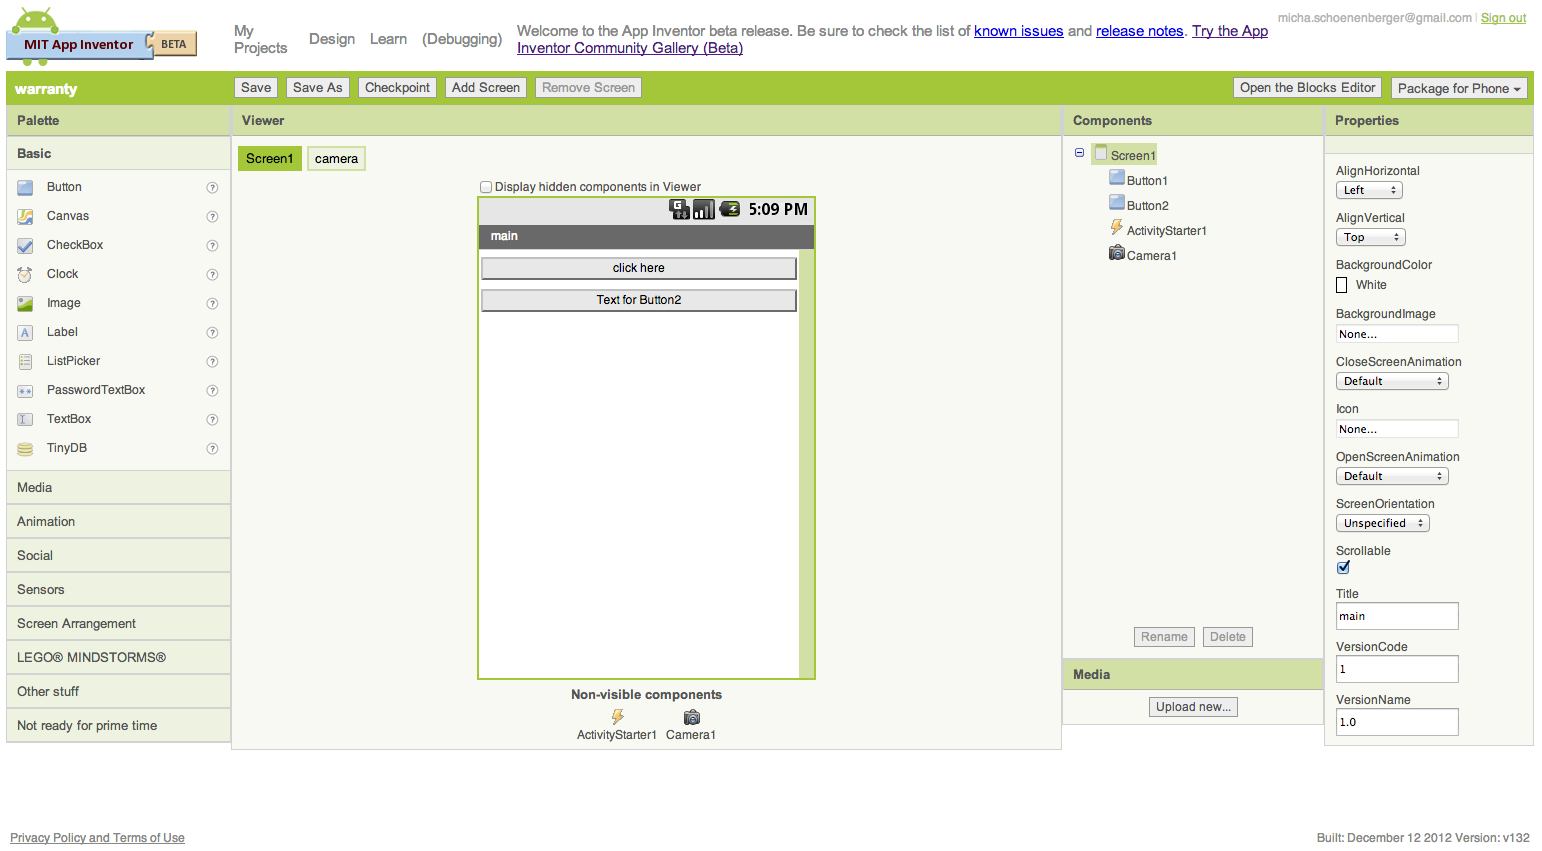
\includegraphics[width=0.9\textwidth]{App_Inventor.png} 
\caption{Screenshot AppInventor}
Quelle: \url{http://beta.appinventor.mit.edu/\#3676309}
\end{figure}


\subsection{Screenshot AppInventor Block Aufbau}
\begin{figure}[h!]
\index{App Inventor}
\label{fig:Screenshot_AppInventor_Block}
\centering
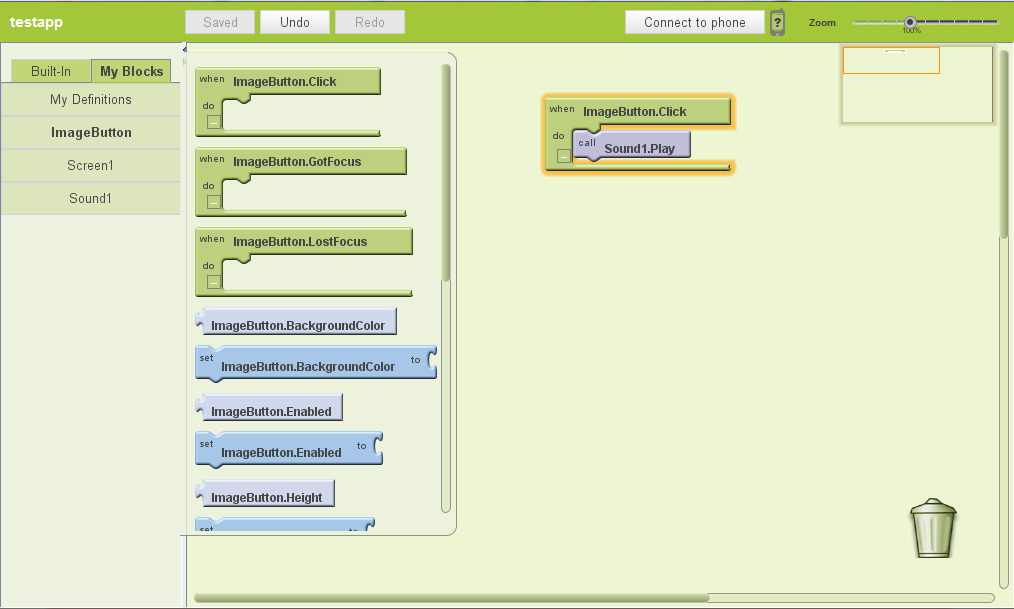
\includegraphics[width=0.9\textwidth]{Screenshot_AppInventor_Block.png} 
\caption{Screenshot AppInventor Block Aufbau }
Quelle: \cite{App_Inventor_Block}
\end{figure}

\newpage
\subsection{Klassendiagramm logische Verkn�pfungen Datenbank}
Auf dem folgenden Klassendiagramm sind die logischen Verkn�pfungen rund um die Datenbank ersichtlich.\\
\begin{figure}[h!]
\index{Klassendiagramm} \index{Datenbank}
\label{fig:class_diagramm_database}
\centering
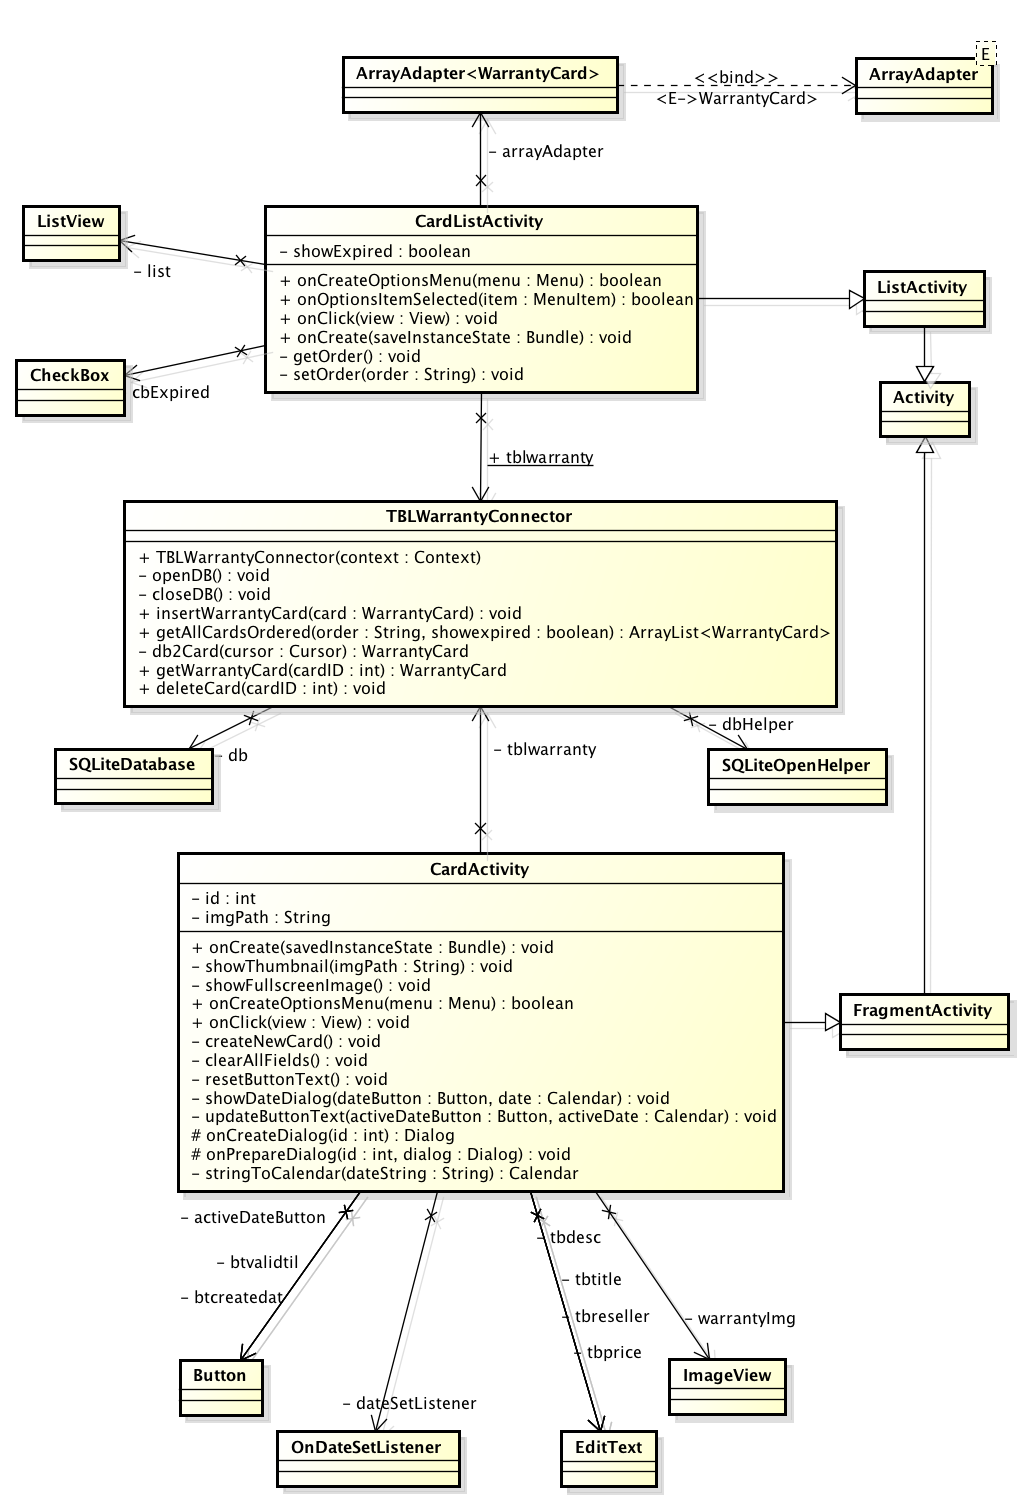
\includegraphics[height=0.8\textheight]{class_diagramm_database.png} 
\caption{Klassendiagramm logische Verkn�pfungen Datenbank}
Klassendiagramm erstellt mit \href{http://www.astah.net}{astah professional} \\
offizielle Website: \url{http://www.astah.net}
\end{figure}



\newpage
\subsection{Klassendiagramm Datenbankschema}
Auf dem folgenden Klassendiagramm ist das Datenbankschema ersichtlich.\\
\begin{figure}[h!]
\index{Klassendiagramm} \index{Datenbank}
\label{fig:class_diagramm_database_scheme}
\centering
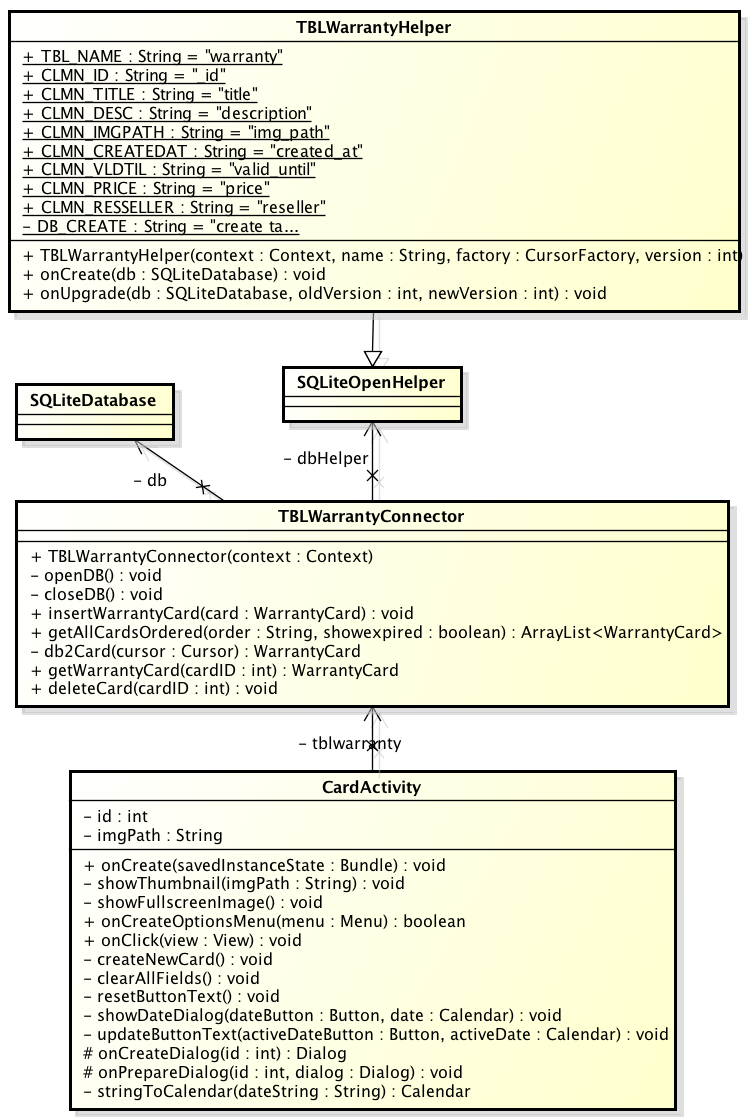
\includegraphics[height=0.8\textheight]{class_diagramm_database_scheme.png} 
\caption{Klassendiagramm Datenbank Schema}
Klassendiagramm erstellt mit \href{http://www.astah.net}{astah professional} \\
offizielle Website: \url{http://www.astah.net}
\end{figure}


